\section{Expresii regulate}
\label{ch:expresii}

Asemeni automatelor finite, expresiile regulate constituie un metalimbaj, adică un limbaj care permite definirea unor alte limbaje. Expresiile regulate au aceeaşi expresivitate ca şi automatele finite şi ca şi gramaticile regulate, adică permit numai definirea limbajelor regulate.

\begin{definitie}
O expresie regulata $ R $ este definită recursiv, astfel:
\begin{itemize}
\item
Şirul vid $\epsilon$ este o expresie regulată, iar limbajul definit de această expresie regulată este limbajul care nu conţine nicio propoziţie. 

\begin{center}
$L(\epsilon)=\{ \}$
\end{center}

\item 
Orice simbol singular $c$ este o expresie regulată, iar limbajul definit de această expresie regulată este limbajul format dintr-o singură propoziţie, şi anume propoziţia $c$. 

\begin{center}
$L(c)=\{ c \}$
\end{center}

\item 
\textbf{Concatenarea:} Dacă $R_1$ şi $R_2$ sunt două expresii regulate, atunci $R1R2$ (se citeşte $R_1$ concatenat cu $R_2$) este o expresie regulată, iar limbajul definit de această expresie regulată este definit astfel: 

\begin{center}
$L(R_1R_2)=\{s_1s_2| s_1 \in R1 \wedge s_2 \in R_2\}$
\end{center}

\item
\textbf{Reuniunea:} Dacă $R_1$ şi $R_2$ sunt două expresii regulate, atunci $R_1|R_2$ (se citeşte $R_1$ sau $R_2$) este o expresie regulată, iar limbajul definit de această expresie regulată este definit astfel:

\begin{center}
$L(R_1|R_2)=L(R_1) \cup L(R_2)$.
\end{center}

\item
\textbf{Închiderea:} Dacă $ R $ este o expresie regulată, atunci $R^*$ este o expresie regulată, iar limbajul definit de această expresie regulată este definit astfel: 

\begin{center}
$L(R^*) = L(\epsilon)\ \cup \ L(R)\ \cup\ L(RR)\ \cup\ L(RRR)\ \cup \dots$
\end{center}

Cu alte cuvinte, limbajul definit de expresia regulată $R^*$ este limbajul format din mulţimea propoziţiilor obţinute prin concatenarea a zero sau mai multe propoziţii, fiecare din $L(R)$.

\item
\textbf{Închiderea nereflexivă:} Dacă $R$ este o expresie regulată, atunci $R^+$ este o expresie regulată, iar limbajul definit de această expresie regulată este definit astfel:

\begin{center}
$L(R^+) = L(R) \cup L(RR) \cup L(RRR) \cup \dots$
\end{center}

Cu alte cuvinte, limbajul definit de expresia regulată $R^+$ este limbajul format din mulţimea propoziţiilor obţinute prin concatenarea a una sau mai multe propoziţii, fiecare din $L(R)$.

$R^+$ este o scriere prescurtată pentru $RR^*$.

\item
\textbf{Opţional:} Dacă $R$ este o expresie regulată, atunci $R?$ este o expresie regulată, iar limbajul definit de această expresie regulată este definit astfel:

\begin{center}
$L(R?) = L(R) | L(\epsilon)$
\end{center}

$R?$ este o scriere prescurtată pentru $R|\epsilon$.
\end{itemize}
\end{definitie}

În general, motoarele de procesare a expresiilor regulate implementate de către aplicaţiile care permit utilizarea lor, permit şi folosirea următoarelor notaţii:

\begin{itemize}
\item
$[ c_{1} c_{2} \dots]$  este o prescurtare pentru  $c_{1} | c_{2} | \dots $.
\item
$[ a_{1}-a_{n} ]$ este o prescurtare pentru $a_{1} | \dots | a_{n} $.
\item
$[ \textasciicircum{} c_{1} c_{2}\dots]$ este o prescurtare pentru $d_{1}|d_{2}|\dots$, unde$ d_{1}, d_{2}, \dots$ sunt toate acele simboluri care nu apar printre $c_{1}, c_{2}, \dots$.
\item 
$.$ este o prescurtare pentru toate şirurile de caractere care sunt formate dintr-un singur caracter, iar acesta nu este sfârşitul de linie.
\end{itemize}

În continuare vor fi prezentate câteva exemple de utilizare a expresiilor regulate pentru a căuta o anumită mulţime de şiruri de caractere într-un text dat.

\begin{itemize} 
\item {Potrivirea unui şir de caractere} 
	\begin{itemize}
	\item
	\textbf{Text}:    Anna Jones and a friend went to lunch 
	\item
	\textbf{Regex}:    went 
	\item
	\textbf{Matches}: Anna Jones and a friend \textbf{went} to lunch 
	\end{itemize}
	
\item {Potrivirea unui singur caracter oarecare, cu excepţia sfârşitului de linie}
	\begin{itemize}
	\item
	\textbf{Text}:       abc def ant cow 	
	\item
	\textbf{Regex}:    a.. 	
	\item
	\textbf{Matches}: \textbf{abc} def \textbf{ant} cow 
	\end{itemize}
 
\item {Potrivirea unui singur caracter dintr-o mulţime dată}
	\begin{itemize}
		\item \textbf{Text:} \space abc def ant cow
		\item \textbf{Regex:} \space $[da]..$
		\item \textbf{Matches:} \space \textbf{abc def ant} cow
		\newline
		
		\item
		\textbf{Text}:	abc pen nda uml
		\item
		\textbf{Regex}:		.[a-d].
		\item
		\textbf{Matches}:	\textbf{abc} pen \textbf{nda} uml
	\end{itemize}

\item {Potrivirea unui spaţiu alb}
	\begin{itemize}
	\item
		\textbf{Text}:	  abc anaconda ant
	\item
		\textbf{Regex}:    a[ ] 
	\item
		\textbf{Matches}:  abc anacond\underline{a }ant
	\end{itemize}

\item {Potrivirea oricărui caracter cu excepţia celor din mulţimea specificată}
	\begin{itemize}
	\item \textbf{Text:} \space abc def ant cow
	\item \textbf{Regex:} \space $[\textasciicircum{} da]..$
	\item \textbf{Matches:} \space a\underline{bc } d\underline{ef } a\underline{nt cow}
	\end{itemize}

\item {Specificarea numărului de potriviri - de zero sau de mai multe ori}
	\begin{itemize}
	\item
	\textbf{Text}: Anna Jones and a friend owned an anaconda
	\item
	\textbf{Regex}: a[a-z]*
	\item
	\textbf{Matches}: \textbf{Anna} Jones \textbf{and a} friend owned \textbf{an anaconda}
	\end{itemize}

\item {Specificarea numărului de potriviri - o data sau de mai multe ori}
\begin{itemize}
\item
\textbf{Text}: Anna Jones and a friend owned an anaconda
\item
\textbf{Regex}: a[a-z]+
\item
\textbf{Matches}: \textbf{Anna} Jones \textbf{and} a friend owned \textbf{an anaconda}
\end{itemize}

\item {Specificarea numărului de potriviri - de zero ori sau o data}
\begin{itemize}
\item
\textbf{Text:} Anna Jones and a friend owned an anaconda
\item
\textbf{Regex:} $an?$
\item
\textbf{Matches:} \textbf{An}n\textbf{a} Jones \textbf{an}d \textbf{a} friend owned \textbf{an} \textbf{a}cond\textbf{a}
\end{itemize}

\item {Specificarea exactă a numărului de potriviri}
\begin{itemize}
\item
\textbf{Text:} Anna Jones and Anne owned an anaconda
\item
\textbf{Regex:} $an\{2\}$
\item
\textbf{Matches:} \textbf{Ann}a Jones and \textbf{Ann}e owned an anaconda
\newline
\item
\textbf{Text:} Anna and Anne lunched with an anaconda annnnnex
\item
\textbf{Regex:}  $an\{2,3\}$
\item
\textbf{Matches:} \textbf{Ann}a and \textbf{Ann}e lunched with an anaconda \textbf{annn}nnex
\end{itemize}

\item{Potrivirea începutului textului în care se face căutarea}
\begin{itemize}
\item \textbf{Text:} an anaconda ate Anna Jones
\item \textbf{Regex:} $\wedge$a
\item \textbf{Matches:} \textbf{a}n anaconda ate Anna Jones
\end{itemize}

\item{Potrivirea sfârşitului textului în care se face căutarea}
\begin{itemize}
\item \textbf{Text:} an anaconda ate Anna Jones
\item \textbf{Regex:} [a-zA-Z]+\textdollar
\item \textbf{Matches:} an anaconda ate Anna \textbf{Jones}
\end{itemize}
\end{itemize}

\subsection{Convenţii de aplicare a expresiilor regulate}

\subsubsection{Precedenţa}

În scrierea expresiilor regulate, precum şi în implementarea motoarelor de expresii regulate, trebuie să se ţină seama de următoarea precedenţă: operatorii închidere, închidere nereflexivă şi opţional au prioritate faţă de concatenare, iar concatenarea are prioritate faţă de reuniune. Pentru o scriere clară şi fără ambiguităţi se pot utiliza parantezele rotunde.

De exemplu, expresia regulată:

\begin{center}
$ab?cd*ef|g$ 
\end{center}

este echivalenta cu:

\begin{center}
$(a(b?)c(d*)ef)|g$
\end{center}

şi reprezintă limbajul format din propoziţiile: \textit{acef}, \textit{g}, \textit{abcef}, \textit{acdddef}, \textit{abcdddef}, \textit{abcdddddef}, ş.a.m.d.

\subsubsection{Prioritatea}

În aplicarea expresiilor regulate asupra unui text dat, poate să apară situaţia în care acelaşi şir de caractere din textul în care se face căutarea, să se potrivească mai multor expresii regulate dintre cele folosite la căutare. De aceea, în general, prioritatea expresiilor regulate folosite la căutare este dată de ordinea în care ele sunt utilizate. 

De exemplu, fie expresiile regulate: 

{\hfil (ab)* }

şi 

{\hfil [a-c]*}

Şirul de caractere "ab" se potriveşte ambelor expresii. Însă, având în vedere ordinea în care au fost date cele două expresii regulate, se va considera că "ab" se potriveşte lui \textit{(ab)*}.

Având în vedere această convenţie, dacă în textul în care se face căutarea folosind o expresie regulată de tipul $R_1|R_2$, există un şir de caractere care se potriveşte atât expresiei regulate $ R_1 $, cât şi expresiei regulate $ R_2 $, atunci se va considera că se potriveşte lui $R_1$.

De asemenea, în aplicarea expresiilor regulate asupra unui text dat, poate să apară şi situaţia în care, în textul în care se face căutarea, să existe şiruri de caractere diferite, care să se potrivească aceleiaşi expresii regulate. În această situaţie, se foloseşte convenţia \textbf {leftmost longest}: dintre toate şirurile de caractere din textul în care se face căutarea, care se potrivesc aceleiaşi expresii regulate, se va alegea cel mai lung dintre ele, căutat de la stânga spre dreapta.

De exemplu, fie expresia regulată:

{\hfil ab|abcd}

Şi fie textul:

"abcd". 

Expresiei regulate se potrivesc următoarele două şiruri de caractere: "ab" sau "abcd". Având în vedere convenţia \textbf {leftmost longest}, aplicarea expresiei regulate va duce la potrivirea celui de-al doilea şir de caractere, care este mai lung.

\subsection{De la expresii regulate la automate finite}

Având în vedere că expresiile regulate şi automatele finite sunt formalisme echivalente, ambele permiţând definirea limbajelor regulate, înseamnă că pentru orice expresie regulată dată se poate construi un automat finit echivalent, adică un automat finit care să definească exact acelaşi limbaj. Pentru fiecare dintre expresiile regulate de bază, din definiţia recursivă a expresiilor regulate, există un automat finit $ \epsilon $ echivalent. Pornind de la aceste echivalenţe, se poate construi automatul finit echivalent oricărei expresii regulate date, indiferent de complexitatea sa. 

În continuare, vor fi prezentate automatele finite $ \epsilon $ echivalente fiecărei expresii regulate de bază. În acest scop se vor folosi următoarele convenţii:

\begin{itemize}
\item
O elipsă reprezintă un automat, care recunoaşte expresia regulată R, sau aceeaşi maşină, dar cu toate stările componente transformate în stări nefinale.
\item
O elipsă este o colecţie de stări şi tranziţii.
\item
Cele două stări marcate reprezintă starea iniţială şi respectiv starea finală, sau starea iniţială şi starea finală, transformată într-o stare nefinală.
\end{itemize}

\begin{figure}[H]
\centering
\begin{tabular}{c|c}
{$\epsilon$}&\begin{tikzpicture}[shorten >=1pt,node distance=2cm,on grid,auto]
  \node[state,initial,accepting]			(0)              			{$ $};
\end{tikzpicture}  \\[6pt] \\
\end{tabular}
\caption{Automatul finit $ \epsilon $ echivalent expresiei regulate $ \epsilon $}
\end{figure}

\begin{figure}[H]
\centering
\begin{tabular}{c|c}
a&\begin{tikzpicture}[shorten >=1pt,node distance=2cm,on grid,auto]
  \node[state,initial]			(0)              			{$ $};
  \node[state,accepting]              (1)   [right of=0] 		{$ $};   

 \path[->]
     (0)	edge 			node	{a} (1)          
  ;
\end{tikzpicture} \\[6pt] \\
\end{tabular}
\caption{Automatul finit $ \epsilon $ echivalent expresiei regulate $ a $}
\end{figure}

\begin{figure}[H]
\centering
\begin{tabular}{c|c}
$R_{1}R_{2}$&\begin{tikzpicture}[shorten >=1pt,node distance=2cm,on grid,auto]

  \node[state,initial]			(0)              			{$ $};

  \node[state]    			(1)   [right  of=0] 	{$ $};

\draw (1,0) ellipse(2cm and 1cm) node at (0.7,0){$R_{1}$};
\draw (3,0) ellipse(2cm and 1cm) node at (3.3,0){$R_{2}$};
  \node[state,accepting]    			(2)   [right  of=1] 	{$ $};
\end{tikzpicture}\\[6pt] \\
\end{tabular}
\caption{Automatul finit $ \epsilon $ echivalent expresiei regulate $ R_{1}R_{2} $}
\end{figure}

\begin{figure}[H]
\centering
\begin{tabular}{c|c}
$R_{1}|R_{2}$&\begin{tikzpicture}[shorten >=1pt,node distance=2cm,on grid,auto]
  \node[state,initial]			(0)              			{$$};
\draw (2.5,1.5) ellipse(2cm and 1cm) node at (2.5,2){$R_{1}$};
  \node[state]    			(1)   [above right  of=0] 	{$$};
  \node[state]    			(2)   [below right  of=0] 	{$$};
  \node[state]    			(3)   [right  of=1] 	{$$};
  \node[state]    			(4)   [right  of=2] 	{$$};
\draw (2.5,-1.5) ellipse(2cm and 1cm) node at (2.5,-2){$R_{2}$};
  \node[state,accepting]              (5)   [below right of=3] 		{$$};   

 \path[->]
     (0)	edge 			node	{$\epsilon$} (2)
           edge			node	{$\epsilon$} (1)
     (3)	edge			node	{$\epsilon$} (5)
     (4)edge			node {$\epsilon$}(5)
  ;
\end{tikzpicture} \\[6pt] \\
\end{tabular}
\caption{Automatul finit $ \epsilon $ echivalent expresiei regulate $ R_{1} | R_{2} $}
\end{figure}

\begin{figure}[H]
\centering
\begin{tabular}{c|c}
R*&\begin{tikzpicture}[shorten >=1pt,node distance=2cm,on grid,auto]

  \node[state,initial]			(0)              			{$$};
\draw (1,0) ellipse(2cm and 1cm) node at (1,0){$R$};
  \node[state]    			(1)   [right  of=0] 	{$$};
  \node[state,accepting]    			(2)   [right  of=1] 	{$$};

\path[->]
     (0)	edge 	[bend left]		node	{$\epsilon$} (2)
     (1)edge [bend left]            	node {$\epsilon$} (0)
  ;
\end{tikzpicture}
\end{tabular}
\caption{Automatul finit $ \epsilon $ echivalent expresiei regulate $ R* $}
\end{figure}

\section{Demonstrarea/Infirmarea regularităţii unui limbaj}

Metoda uzuală folosită pentru a demonstra că un limbaj este regular constă în a construi un automat cu stări finite sau o expresie regulară care să accepte limbajul respectiv. Cum se poate însp demonstra că un limbaj nu este regular? În continuare vor fi oferite trei astfel de metode/criterii: principiul cuiburilor de porumbei, lema pompării și teorema MyHill-Nerode à la Brzozowski.

\subsection{Principiul cuiburilor de porumbei}

Principiul cuiburilor de porumbei afirmă faptul că dacă \textit{n} porumbei zboară spre \textit{m} cuiburi şi dacă \textit{n>m}, atunci cel puţin un cuib va avea doi sau mai mulţi porumbei.

Acest principiu poate fi aplicat şi automatelor finite. Deoarece acestea au un număr finit de stări şi deoarece, în general,  există un număr infinit de propoziţii care sunt acceptate de către automat, atunci trebuie să existe cel puţin o stare la care automatul, în analiză, se întoarce de două sau de mai multe ori. În cadrul acestei analogii, stările automatului sunt cuiburile, iar simbolurile propoziţiilor de la intrare sunt porumbeii.

Fie limbajul format din orice succesiune de 0 şi 1 care începe cu un 1, continuă apoi cu unul sau mai mulţi de zero, iar la sfârşit are un 1. Mulţimea propoziţiilor acestui limbaj este infinită, cuprinzând succesiunile de simboluri: $ 101 $, $ 1001 $, $ 10001 $, $ 10\dots01 $. Cu toate acestea, mulţimea stărilor automatului este finită. Prin urmare, conform principiului cuiburilor de porumbei, trebuie să există o stare $ q_m $ astfel încât, în analiza a două succesiuni de simboluri $ 10^{p} $ şi $ 10^{q} $, cu $ p \neq q $, automatul va ajunge în aceeaşi stare $ q_m $.

Principiul cuburilor de porumbei poate fi folosit pentru a demonstra că un limbaj dat nu este regulat. Vom exemplifica acest lucru pentru următorul limbaj:

$ L = \{ a^n b^n | n \geq 1  \} $

Dacă ar exista un automat finit care să definească acest limbaj, atunci el ar trebui ca, pe măsură ce analizează şirul de la intrare, să ţină minte numărul de simboluri de $ a $ pe care le-a analizat. Valorile pe care le poate lua numărul de simboluri de $ a $ sunt infinite şi deci automatul ar trebui să poată să gestioneze un număr infinit de posibilităţi. Acest lucru însă nu se poate face cu un număr finit de stări. Deci limbajul dat este un limbaj neregulat.

În continuare se va demonstra acest lucru folosind principiul cuiburilor de porumbei. Demonstraţia va fi o demonstraţie prin reducere la absurd.

\begin{proof}
Presupunem că limbajul $ L $ este un limbaj regulat. Atunci, înseamnă că există un automat finit $AF=(\{ a, b \}, Q, F, q_{0}, f)$ care acceptă acest limbaj. Considerăm $ f^* (q_0, a^i) $ pentru $ i $ egal cu $ 1, 2, \dots $. Deoarece $ i $, numărul de $ a $, poate lua un număr infinit de valori, şi deoarece mulţimea de stări din automat este finită, atunci, conform principiului cuiburilor de porumbei, există o stare $ q_k $ astfel încât:

$ f^* (q_0, a^m) = q_k $ şi $ f^* (q_0, a^n) = q_k $, cu $ m \neq n $.

Dar, deoarece automatul accepta şirurile de forma $ a^n b^n $, atunci este obligatoriu să fie adevărat că:

$ f^* (q_k, b^n) = q_f \in F $.

Pe baza relaţiile scrise mai sus, se poate deduce că:

$ f^* (q_0, a^m b^n) = f^* (f^* (q_0, a^m), b^n) = f^* (q_k, b^n) = q_f \in F$ 

Dar acest lucru înseamnă că automatul accepta şi şirurile de forma $ a^m b^n $, cu $ m \neq n $, ceea ce contrazice presupunerea iniţială cum că el accepta limbajul $ L $. Deci presupunerea iniţială este falsă şi deci $ L $ este un limbaj neregulat.
\end{proof}

\subsection{Lema pompării pentru limbajele regulare}

\begin{theorem}
\textbf{[Lema pompării]}Dacă L este un limbaj regulat, atunci există un număr natural $N \geq 1$, astfel încât $\forall$ propoziţie w $\in$ L, unde |w| $\geq$ N, $\exists$ x, y, z astfel încât w=xyz, şi :
\begin{itemize}
\item
$|xy| \leq N$
\item
y $\neq$ $\epsilon$
\item
$\forall$ q $\geq$ 0, $xy^{q}z$ $\in$ L.
\end{itemize}
\end{theorem}

Cu $ |x| $ s-a notat lungimea propoziţiei $ x $, iar cu $ x^q $ s-a notat concatenarea propoziţiei $ x $ cu ea însăşi de un număr de ori egal cu $ q $.

Cu alte cuvinte, lema pompării enunţă faptul că dacă $ L $ este un limbaj regulat, atunci există un număr natural $ N $ care este cel puţin egal cu $ 1 $, astfel încât, pentru orice propoziţie $ w $ din limbajul $ L $, care are lungimea cel puţin egală cu $ N $, există o formă de scriere prin concatenarea a trei subşiruri $ x, y, z $, cu proprietăţile că lungimea subşirului $ xy $ este cel mult egală cu $ N $, iar lungimea subşirului $ y $ este cel puţin egală cu 1. În aceste condiţii, subşirul $ y $ poate fi pompat ori de câte ori între $ x $ şi $ z $ ($ xyy \dots yz $) sau chiar poate fi eliminat ($ xz $), iar propoziţiile obţinute astfel aparţin şi ele limbajului $ L $.

\begin{proof}
Dacă $ L $ este un limbaj regulat, atunci înseamnă că există un automat finit determinist care îl defineşte. Presupunem că automatul are un număr $ n + 1 $ de stări şi că acestea sunt etichetate cu $ q_0, q_1, \dots, q_n $. 

Fie atunci o propoziţie $ w \in L $, astfel încât $ |w| \geq m = n +1 $ şi fie $ q_0, q_i, q_j, \dots, q_f $ succesiunea de stări prin care automatul trece în analiza propoziţiei $ w $ (evident $ q_0 $ este starea iniţială, iar $ q_f $ este o stare finală). Numărul de stări din cadrul acestei succesiuni de stări este egal cu lungimea şirului $ w $ plus 1, deoarece pentru a accepta un număr de simboluri egale cu lungimea lui $ w $, este nevoie de acelaşi număr de tranziţii, iar numărul de stări necesare pentru a forma aceste tranziţii este mai mare cu 1. Acest lucru implică faptul că cel puţin o stare din succesiunea $ q_0, q_i, q_j, \dots, q_f $ se repetă. Prin urmare, succesiune de stări poate fi rescrisă $ q_0, q_i, q_j, \dots, q_r, \dots, q_r, \dots, q_f $. 

Această scriere a succesiuni de stări prin care trece automatul în analiza şi acceptarea propoziţiei $ w $, indică că aceasta poate fi scrisă ca o concatenare a trei subşiruri $ x, y, z $, astfel încât:

\begin{itemize}
\item
şirul $ x $ este prima parte a propoziţiei $ w $, pentru analiza căreia automatul trece prin succesiunea $ q_0, q_i, q_j, \dots, q_r$, şi se poate scrie:

$ (q_0,x) \vdash^* (q_r, \epsilon)  $ sau $ f^*(q_0, x) = q_r $
\item
şirul $ y $ este partea de mijloc a propoziţiei $ w $, pentru analiza căreia automatul trece prin succesiunea $ q_r, \dots, q_r$,  şi se poate scrie:

$ (q_r,y) \vdash^+ (q_r, \epsilon)  $ sau $ f^*(q_r, y) = q_r $
\item
iar şirul $ z $ este ultima parte a propoziţiei $ w $, pentru analiza căreia automatul trece prin succesiunea $q_r, \dots, q_f $, şi se poate scrie:

$ (q_r,z) \vdash^+ (q_f, \epsilon)  $ sau $ f^*(q_r, z) = q_f $.
\end{itemize}

De aici rezultă că:

\begin{itemize}
\item
$ |xy| \leq n + 1 = m $ deoarece am presupus ca singura stare care se repetă în analiza propoziţiei $ w $ este $ q_r $ şi deci, în rest, stările sunt distincte. Prin urmare, pentru şirurile $ x, y $ se pot analiza un număr maxim de simboluri egal cu numărul maxim de stări care pot fi implicate în analiză, adică $ n + 1 $;
\item
$ |y| \geq 1 $, deoarece s-a arătat că starea $ q_r $ trebuie să se repete, şi deci între cele două apariţii ale acestei stări va fi acceptat cel puţin un simbol (în cazul în care a doua apariţie a lui $ q_r $ urmează imediat după prima).
\end{itemize}

Totodată, având în vedere relaţiile de mai sus, se poate scrie că:

\begin{enumerate}
\item
$ (q_0,xz) \vdash^* (q_r, z) \vdash^+ (q_f, \epsilon) $, ceea ce înseamnă că $ xz \in L $;
\item
$ (q_0,xy^{2}z) \vdash^* (q_r, y^{2}z) \vdash^+ (q_r, yz) \vdash^+ (q_r, z) \vdash^+ (q_f, \epsilon)$, ceea ce înseamnă că $ xy^{2}z \in L $;
\item
în acelaşi mod se poate arăta că $ xy^{3}z \in L $ şi $ xy^{4}z \in L $, şi, în general, $ xy^{q}z \in L $, pentru orice număr natural $ q $.
\end{enumerate}

Cu aceasta, demonstraţia teoremei s-a încheiat.
\end{proof}

Lema pompării este folosită pentru a demonstra că un limbaj dat nu este un limbaj regulat. Această demonstraţie se face totdeauna prin reducere la absurd. 

În continuare se va exemplifica modul în care se utilizează această teoremă pentru a arăta că un limbaj dat nu este regulat și anume se va arăta că limbajul:

L=\{$a^{n}$ $b^{n}$| n$\geq$ 1\}

nu este un limbaj regular.

\begin{proof}
Presupunem că limbajul este unul regular. Atunci, înseamnă că i se poate aplica lema pompării și anume: există un număr natural $N \ge 1$ astfel încât pentru orice propoziție $w \in L$ care are lungimea cel puțin egală cu $N$ se îndeplinesc afirmațiile lemei.

Fie w = $a^{N}$ $b^{N}$. Atunci, indiferent de modul în care propoziția $w$ este scrisă ca și o concatenare de trei șiruri $xyz$, se îndeplinesc afirmațiile teoremei. Având în vedere că, în conformitate cu lema pompării, $|xy| \le N$ și având în vedere felul în care l-am ales pe $w$, înseamnă că $y$ poate lua următoarele forme:

y=$a^{i}$, $1 \leq |y| \leq N$.

Însă, pentru că $|xy| \leq N$:

$x=a^{j}$, cu condiția că $i+j \leq N$.

Cu aceste observații, rezultă că șirul $w$ are forma:  

$w=a^{j}$ $a^{i}$ $a^{N-(i+j)}$ $b^{N}$.

În aceste condiții, lema afirmă că pentru orice număr natural $q \ge 0$, $x y^q z \in L$.

Pentru că demonstrația pe care o facem este una prin reducere la absurd, căutăm o valoare a lui $q$ astfel încât: 

$w^{`}$= $a^{j}$ ${a^{i}}^{q}$ $a^{N-(i+j)}$ $b^{N}$ $\nexists$ L, 

unde  $w^{`}$ este şirul pompat. 

Se observă că pentru $q=0$: 

$w^{`}$= $a^{j}$ $a^{N-(i+j)}$ $b^{N}$ = $a^{N-i}$ $b^{N} \notin L$.

Am ajuns astfel la o contradicție, prin urmare, limbajul $L$ nu este un limbaj regular.
\end{proof}

Lema pompării nu poate fi folosită pentru a demonstra că un limbaj este regulat, deoarece reciproca ei nu este adevărată: există limbaje care pot fi pompate, dar care, totuşi, nu sunt regulate. În continuare se va exemplifica acest lucru pe baza limbajului:

L = \{ uvwxy : u,y $\in$ \{0,1,2,3\}* ; v, w, x $\in$ \{0,1,2,3\} $\wedge$ ( v = w $\vee$ v=x $\vee$ x=w ) \} $\cup$ \{ w : w $\in$ \{ 0,1,2,3 \}* $\wedge$  exact 1/7 simboluri din w să fie 3 \}.

Cu alte cuvinte, limbajul $L$ este reprezentat de mulțimea tuturor propozițiile construite pe baza alfabetului \{0,1,2,3\} care au un subșir de trei simboluri, în care un același simbol apare de două ori, precum și toate propozițiile formate pe baza aceluiași alfabet în care exact $1/7$ dintre simboluri sunt simbolul 3.

Acest limbaj nu este un limbaj regular (spre exemplu $(013)^{3m}(012)^{i} \in L$ dacă și numai dacă $i=4m$), dar poate fi pompat pentru N având valoarea 5. Fie deci o propoziție $w$ care are lungimea cel puțin egală cu 5. Deoarece alfabetul limbajului are numai 4 simboluri, înseamnă că cel puțin două dintre primele 5 simboluri sunt identice, iar aceste două simboluri identice sunt separate de cel mult trei simboluri. 

\begin{itemize}
\item
Dacă cele două simboluri identice nu sunt separate de niciun simbol sau sunt separate de un singur simbol, atunci se poate pompa oricare dintre celelalte două simboluri din propoziție, fără a afecta subșirul care conține simbolurile duplicate.

Variantele posibile pot fi schematizate astfel:

$\textbf{aa}bcd$, $\textbf{a}b\textbf{a}cd$, $b\textbf{aa}cd$, $b\textbf{a}c\textbf{a}d$, $bc\textbf{aa}d$, $bc\textbf{a}d\textbf{a}$, $bcd\textbf{aa}$, etc.

Spre exmplu, pentru prima variantă, se poate pompa simbolul $c$ sau simbolul $d$, obținându-se:

$\textbf{aa}bc^q d$ sau $\textbf{aa}bcd^q$.

Se observă că subșirul care conține simbolurile identice ($aab$) nu este afectat și deci propozițiile obținute aparțin limbajului $L$ (având un subșir de trei simboluri dintre care două sunt identice).
\item
Dacă cele două simboluri identice sunt separate de două sau de trei simboluri, atunci pot fi pompate două dintre simbolurile care le separă. Pomparea va duce la obținerea unui subșir de trei simboluri, dintre care două sunt identice.

Variantele posibile pot fi schematizate astfel:

$\textbf{a}bc\textbf{a}d$, $\textbf{a}bcd\textbf{a}$, $b\textbf{a}cd\textbf{a}$, etc.

Spre exemplu, pentru prima variantă, se poate pompa grupul $bc$, obținându-se:

$a(bc)^q ad$.

Este evident că orice repetare a grupului $bc$ va duce la crearea unui subșir de trei simboluri dintre care două sunt identice.
\end{itemize}

Exemplul de mai sus ne arată că lema pompării ne dă o condiţie necesară, dar nu și suficientă, pentru a arata că un limbaj este regular.

\subsection{Teorema Myhill-Nerode à la Brzozowski}

Janusz Antoni Brzozowski a definit în anul 1964 operația de derivare a unui limbaj, definind operația de derivare a unei expresii regulare. Derivata unui limbaj $L$ în raport cu un simbol $c$ este un nou limbaj obținut prin aplicarea următoarelor două operații:

\begin{enumerate}
\item
Se rețin toate propozițiile limbajului $L$ care încep cu simbolul $c$.
\item
Se elimină simbolul $c$ din poate aceste propoziții.
\end{enumerate}

Formal, derivata unui limbaj $L$ în raport cu un simbol $c$ se definește astfel:

$\frac{d}{ dc}$L = \{ v | cv $\in$ L \}.

Oferim mai jos câteva exemple de derivate pentru niște expresi regulare.

$\frac{d}{da}$ ab*a = b*a

$\frac{d}{db}$ ab*a =$\emptyset$

$\frac{d}{db}$ b*a = b*a

Utilizând operația de derivare, este foarte ușor de observat și de demonstrat că derivata unui limbaj regular este tot un limbaj regular. Orice limbaj regular poate fi definit prin intermediul unui automat cu stări finite. Dar, operația de derivare, prin care se obține limbajul derivat, corespunde schimbării stării inițiale a automatului finit care definește limbajul supus operației de derivare. Prin urmare și derivata unui limbaj este definită printr-un automat cu stări finite, ceea ce înseamnă că este un limbaj regular.

Utilizând un raționament similar, se poate observa și demonstra cum că un limbaj regular are un număr finit de derivate distincte. Având în vedere că operația de derivare a unui limbaj înseamnă de fapt schimbarea stării inițiale a automatului cu stări finite care definește limbajul supus derivării și având în vedere că numărul de stări ale unui automat este finit, rezultă că numărul de derivate posibile este maxim egal cu numărul de stări ale automatului și deci este un număr finit.

Reciproca afirmației anterioare este și ea adevărată: dacă un limbaj are un număr finit de derivate distincte, atunci el este un limbaj regular. Această afirmație este numită Teorema Myhill-Nerode à la Brzozowski.

În continuare se va exemplifica modul în care această teoremă poate fi utilizată pentru a arăta că un limbaj dat nu este regular.

Fie limbajul:

L = \{ $a^{i} b^{i}$ | $\forall$ i $\in \mathbb{N}$ \}.

Să se arate că $L$ nu este un limbaj regular.

\begin{proof}

Pentru a arăta că limbajul nu este regular, se va arăta că numărul de derivate distincte ale limbajului este infinit. De exemplu, se va deriva limbajul dat în raport cu $a^n$. Se va obține:

$\frac{d}{da^{n}}$ $a^{i+n}$ $b^{i+n}$ = $a^{i}$ $b^{i+n}$, $\forall i,n \in \mathbb{N}$.

Depinzând de $n$, este evident că numărul de derivate distincte obținute este infinit. Prin urmare, limbajul nu este unul regular.
\end{proof}

Aplicând aceeași logică și în cazul limbajului:

L = \{ $a^{i} b$ | $\forall$ i $\in \mathbb{N}$ \}.

vom obține că:
 
$\frac{d}{da^{n}}$ $a^{i+n}$b = $a^{i}b $ 

Numărul de derivate este tot infinit, însă ele nu sunt distincte. Prin urmare limbajul este unul regular.
  
Vom exemplifica utilizarea teoremei și pentru limbajul $L$ folosit în secțiunea anterioară pentru a arăta că reciproca lemei pompării nu este adevărată.

Fie limbajul:

L = \{ uvwxy : u,y $\in$ \{0,1,2,3\}* ; v, w, x $\in$ \{0,1,2,3\} $\wedge$ ( v = w $\vee$ v=x $\vee$ x=w ) \} $\cup$ \{ w $\in$ \{0,1,2,3\}*| ( $n_{\{0,1,2\}}(w) = 6*n_{\{3\}} (w)$ \}.

Să se demonstreze că acest limbaj nu este un limbaj regular.

\begin{proof}
Notând cu $C$ a doua submulțime a propozițiilor din limbajul $L$, vom calcula derivata:

$\frac{d}{d(0123)^{i}}$C = \{w $\in$ \{0123\}* | $n_{\{0,1,2\}}((0123)^{i}w) = 6*n_{\{3\}}((0123)^iw)$ \} = 

\{w $\in$ \{0123\}* | $n_{\{0,1,2\}}((0123)^{i}) + n_{\{0,1,2\}}(w) = 6*(n_{\{3\}}((0123)^{i}) +  n_{\{3\}}(w)) \}$ =

\{w $\in$ \{0123\}* | $3*i + n_{\{0,1,2\}}(w) = 6*i + 6*n_{\{3\}}(w)$ \} =

\{w $\in$ \{0123\}* | $n_{\{0,1,2\}}(w)  = 3*i + 6*n_{\{3\}}(w)$ \}.

Aceste limbaje sunt distincte, deoarece, spre exemplu, pentru fiecare valoare a lui $i$ derivata $\frac{d}{d(0123)^{i}}C$ conține șirul $(012)^i$, însă niciuna dintre celelate derivate nu conține acest șir. Prin urmare, $L$ are un număr infinit de derivate distincte și deci nu este un limbaj regular.
\end{proof}

\subsection{Exerciţii}

\begin{enumerate}
\item
Să se definească expresiile regulate care să permită recunoaşterea următorilor atomi lexicali, pentru limbajul C\# şi să se verifice folosind \url{http://regexr.com/}:

\begin{itemize}
\item
variabilele:

\begin{verbatim}
([A-Za-z][A-Za-z_0-9]*)|([_][A-Za-z_0-9]+)
\end{verbatim}

\item
comentariile de o singură linie:

\begin{verbatim}
(\/\/).*
\end{verbatim}

\item
comentariile de mai multe linii:

\begin{verbatim}
\/\*([^*]|[\r\n]|(\*+([^*/]|[\r\n])))*\*+\/
\end{verbatim}

\item
constantele de tip numere întregi:

\begin{verbatim}
[+-]?[0-9]+
\end{verbatim}

\item
constantele de tip numere reale:

\begin{verbatim}
[+-]?[0-9]+[.][0-9]+
\end{verbatim}

\item
constantele de tip caracter:

\begin{verbatim}
'(.|\\n|\\t)'
\end{verbatim}

\item
constantele de tip şir de caractere:
\begin{verbatim}
\"((\\\")|[^\"])*\"
\end{verbatim}
\end{itemize}

\item
Să se construiască expresia regulată şi automatul finit determinist echivalente cu gramatica regulată:
\begin{itemize}
\item 
$\Sigma = \{$a, b\}
\item
$V_{N}$ = \{S, A, B\}
\item
P=\{ S $\rightarrow$ abA, A $\rightarrow$ baB, B $\rightarrow$ aA| bb \}
\end{itemize}

Propoziţiile din limbajul generat de această gramatică, vor avea forma următoarele forme (de la cea mai simplă, până la cea mai complexă):
\begin{itemize}
\item
ab\textbf{ba}bb
\item
ab\textbf{ba\underline{aba}}bb
\item
ab\textbf{ba\underline{aba}\underline{aba}}bb
\item
ab\textbf{ba\underline{aba}...\underline{aba}}bb
\end{itemize}

Rezultă deci că expresia regulată echivalentă este:

\begin{verbatim}
abba[aba]*bb
\end{verbatim}

Automatul finit echivalent este:

\begin{figure}[H]
\centering
\begin{tikzpicture}[shorten >=1pt,node distance=1.5cm,on grid,auto]
\node[initial, state] (0) {$q_0$};
\node[state] (1) [right of=0] {$q_1$};
\node [state, accepting] (2) [right of=1] {$q_2$};
\node [state] (3) [right of=2] {$q_3$};
\node [state] (4) [right of=3] {$q_4$};
\node [state] (5) [right of=4] {$q_5$};
\node [state, accepting] (6) [right of=5] {$q_6$};

\path [->]
	(0) edge	node{a}(1)
	(1) edge	node{b}(2)
	(2)edge 	node{b}(3)
	(4) edge [bend left] node{a} (2)
	(3)edge	node{a}(4)
	(4)edge 	node{b}(5)
	(5)edge	node{b}(6)
	;
\end{tikzpicture}
\end{figure}

\item
Să se construiască expresia regulată şi gramatica echivalente cu automatul finit determinist:

\begin{figure}[H]
\centering
\begin{tikzpicture}[shorten >=1pt,node distance=1.5cm,on grid,auto]
\node[initial, state] (0) {$q_0$};
\node[state, accepting] (1) [right of=0] {$q_1$};
\node [state] (2) [right of=1] {$q_2$};

\path [->]
	(0) edge [loop above] 	node{b}()
	(0) edge	node{a}(1)
	(1) edge	node{b}(2)
	(2)edge [loop above]	node{b}()
	(2)edge [bend left]	node{a}(0)
	;
\end{tikzpicture}
\end{figure}

Propoziţiile din limbajul generat de această gramatică, vor avea forma următoarele forme (de la cea mai simplă, până la cea mai complexă):
\begin{itemize}
\item
a
\item
\textbf{b} a
\item
\textbf{bb} a
\item
\textbf{b$\dots$b} a
\item
\textbf{b$\dots$b} a \underline{b b$\dots$b a} \textbf{b$\dots$b} a
\item
\textbf{b$\dots$b} a \underline{b b$\dots$b a} \textbf{b$\dots$b} a \underline{b b$\dots$b a} \textbf{b$\dots$b} a
\item
$\dots$
\end{itemize}

Rezultă deci că expresia regulată echivalentă este:
\begin{verbatim}
b* a (b + a b* a)*
\end{verbatim}

Gramatica regulată echivalentă este:

\begin{itemize}
\item 
$\Sigma = \{$a, b\}
\item
$V_{N}$ = \{S, A, B\}
\item
P=\{ S $\rightarrow$ bS | aA | a, A $\rightarrow$ bB, B $\rightarrow$ bB| aS \}
\end{itemize}

\item 
Să se genereze automatul $\epsilon$ care verifică expresia regulată:	0?[1-3]+ | (01)+ .

0? se înlocuieşte cu 0|$\epsilon$.

Atunci expresia regulată devine:		((0|$\epsilon$)[1-3]+) | (01)+

\begin{figure}[H]
\centering
\begin{tikzpicture}[shorten >=1pt,node distance=1.5cm,on grid,auto] 
\node [state, initial] (0) {$q_{0}$};
\node [state] [above right of=0] (1) {$q_{1}$};
\node [state] [right of=1] (2) {$q_{2}$};
\node [state, accepting] [below right of=2] (5) {$q_{5}$};
\node [state] [below right of=0] (3) {$q_{3}$};
\node [state] [right of=3] (4) {$q_{4}$};

\path[->]
	(0) edge node{$\epsilon$} (1)
	(0)edge node {$\epsilon$} (3)
	(1) edge node{0}(2)
	(2) edge node{$\epsilon$} (5)
	(3)edge node {$\epsilon$} (4)
	(4) edge node {$\epsilon$} (5)
	;
\end{tikzpicture}
\caption{Automatul pentru expresia:  0|$\epsilon$}
\end{figure}

\begin{figure}[H]
\centering
\begin{tikzpicture}[shorten >=1pt,node distance=1.5cm,on grid,auto] 
\node [state, initial] (0) {$q_{0}$};
\node[state, accepting] [right of=0] (1) {$q_{1}$};
\path[->]
	(0)edge node{0}(1)
	;
\end{tikzpicture}
\caption{Automatul pentru 0}
\end{figure}

\begin{figure}[H]
\centering
\begin{tikzpicture}[shorten >=1pt,node distance=1.5cm,on grid,auto] 
\node [state, initial] (0) {$q_{0}$};
\node[state, accepting] [right of=0](1) {$q_{1}$};
\path[->]
	(0)edge node{$\epsilon$}(1)
	;
\end{tikzpicture}
\caption{Automatul pentru $\epsilon$}
\end{figure}

\begin{figure}[H]
\centering
\begin{tikzpicture}[shorten >=1pt,node distance=2cm,on grid,auto] 
\node [state, initial] (0) {$q_{0}$};
\node[state, accepting] [right of=0](1) {$q_{1}$};
\path[->]
	(0)edge node{1|2|3}(1)
	;
\end{tikzpicture}
\caption{Automatul pentru [1-3]}
\end{figure}

\begin{figure}[H]
\centering
\begin{tikzpicture}[shorten >=1pt,node distance=2cm,on grid,auto] 
\node [state, initial] (0) {$q_{0}$};
\node[state, accepting] [right of=0](1) {$q_{1}$};
\path[->]
	(0)edge node{1|2|3}(1)
	(1)edge [bend left] node{$\epsilon$}(0)
	;
\end{tikzpicture}
\caption{Automatul pentru [1-3]+}
\end{figure}

\begin{figure}[H]
\centering
\begin{tikzpicture}[shorten >=1pt,node distance=2cm,on grid,auto] 
\node [state, initial] (0) {$q_{0}$};
\node [state] (1) [right of=0]{$q_{1}$};
\node[state, accepting] [right of=1](2) {$q_{2}$};
\path[->]
	(0)edge node{0}(1)
	(1)edge node{1}(2)
	;
\end{tikzpicture}
\caption{Automatul pentru (01)}
\end{figure}

\begin{figure}[H]
\centering
\begin{tikzpicture}[shorten >=1pt,node distance=2cm,on grid,auto] 
\node [state, initial] (0) {$q_{0}$};
\node [state] (1) [right of=0]{$q_{1}$};
\node[state, accepting] [right of=1](2) {$q_{2}$};
\path[->]
	(0)edge node{0}(1)
	(1)edge node{1}(2)
	(2)edge [bend left] node{$\epsilon$}(0)
	;
\end{tikzpicture}
\caption{Automatul pentru (01)+}
\end{figure}

\begin{figure}[H]
\centering
\begin{tikzpicture}[shorten >=1pt,node distance=2cm,on grid,auto] 
\node[state, initial] (0) {$q_{0}$};
\node[state] [above right of=0] (1) {$q_{1}$};
\node [state] [right of=1] (2) {$q_{2}$};
\node [state] [below of=1] (3) {$q_{3}$};
\node [state] [right of=3] (4) {$q_{4}$};
\node [state] [above right of=4] (5) {$q_{5}$};
\node[state] [right of=5](6) {$q_{6}$};
\node [state, accepting] [below right of=6] (11) {$q_{11}$};
\node [state] [below of=3] (7) {$q_{7}$};
\node [state] [right of=7] (8) {$q_{8}$};
\node [state] [right of=8] (9) {$q_{9}$};
\node [state] [right of=9] (10) {$q_{10}$};

\path[->]
	(0)edge node{$\epsilon$}(1)
	(0)edge node{$\epsilon$}(3)
	(0)edge node{$\epsilon$}(7)
	(3)edge node{$\epsilon$}(4)
	(2)edge node{$\epsilon$}(5)
	(7)edge node{$\epsilon$}(8)
	(4)edge node{$\epsilon$}(5)
	(6)edge node{$\epsilon$}(11)
	(10)edge node{$\epsilon$}(11)
	(1)edge node{0}(2)
	(8)edge node{0}(9)
	(9)edge node{1}(10)
	(5)edge node{1$\dots$3}(6)
	(6)edge[bend left] node{$\epsilon$}(5)
	(10)edge[bend left] node{$\epsilon$}(8)
	;
	
\end{tikzpicture}
\caption{Automatul epsilon pentru 0?[1-3]+|(01)+}
\end{figure}

\begin{figure}[H]
\centering
\begin{tikzpicture}[shorten >=1pt,node distance=2cm,on grid,auto] 
\node [state, initial] (6) {$q_{6}$};
\node[state] [above right of=6] (1) {$q_{1}$};
\node [state, accepting] [below right of=1] (5) {$q_{5}$};
\node [state] [below right of=6] (8) {$q_{8}$};
\node [state, accepting] [right of=8] (9) {$q_{9}$};
\path [->]
	(6)edge node{0} (1)
	(6) edge node{1$\dots$3}(5)
	(6)edge node{0}(8)
	(1) edge node{1$\dots$3}(5)
	(8)edge node{1}(9)
	;
\end{tikzpicture}
\caption{Automatul pentru  0?[1-3]+|(01)+ fără stări $\epsilon$}
\end{figure}

\item
Fie expresia regulată: $0(00)^*(10)+$. Construiţi automatul finit epsilon care acceptă limbajul definit de această expresie regulată.

\begin{itemize}
\item[Pas 1:] $0$

\begin{figure}[H]
\centering
\begin{tikzpicture}[shorten >=1pt,node distance=3cm,on grid,auto]

  \node[state,initial]	(0)              		{$S_{0}$};
  \node[state,accepting]   		(1)   	[right of=0] 	{$S_{1}$};  
 \path[->]
     (0)	edge 						node	{$0$} (1)
  ;
\end{tikzpicture}
\caption{$0$}
\end{figure}
\end{itemize}

\item[Pas 2:] $(00)^*$

\begin{figure}[H]
\centering
\begin{tikzpicture}[shorten >=1pt,node distance=3cm,on grid,auto]

  \node[state,initial]	(0)              		{$S_{2}$};
  \node[state]			(1)   	[right of=0] 	{$S_{3}$};  
  \node[state,accepting](2)   	[right of=1] 	{$S_{4}$};
 \path[->]
     (0)	edge 						node	{$0$} (1)
     (1)	edge 						node	{$0$} (2)
     (2)	edge 	[bend left =30]		node{$\epsilon$} (0)
  ;
\end{tikzpicture}
\caption{$(00)^*$}
\end{figure}

\item[Pas 3:]
Contopim $S1$ cu $S2$ si obtinem:

\begin{figure}[H]
\centering
\begin{tikzpicture}[shorten >=1pt,node distance=3cm,on grid,auto]

  \node[state,initial]	(0)              		{$S_{0}$};
  \node[state]			(1)   	[right of=0] 	{$S_{1}$};  
  \node[state](2)   	[right of=1] 	{$S_{3}$};
  \node[state,accepting](3)   	[right of=2] 	{$S_{4}$};
 \path[->]
     (0)	edge 						node	{$0$} (1)
     (1)	edge 						node	{$0$} (2)
     (2)	edge 						node	{$0$} (3)
     (3)	edge 	[bend left =30]		node{$\epsilon$} (1)
  ;
\end{tikzpicture}
\caption{$0(00)^*$}
\end{figure}

\item[Pas 4:] $(10)^*$

\begin{figure}[H]
\centering
\begin{tikzpicture}[shorten >=1pt,node distance=3cm,on grid,auto]

  \node[state,initial]	(0)              		{$S_{5}$};
  \node[state]			(1)   	[right of=0] 	{$S_{6}$};  
  \node[state,accepting](2)   	[right of=1] 	{$S_{7}$};
 \path[->]
     (0)	edge 						node	{$1$} (1)
     (1)	edge 						node	{$0$} (2)
     (2)	edge 	[bend left =30]		node{$\epsilon$} (0)
  ;
\end{tikzpicture}
\caption{$(10)^*$}
\end{figure}

\item[Pas 5:] 
Contopim starile $q_{1}$ cu $q_{5}$.

\begin{figure}[H]
\centering
\begin{tikzpicture}[shorten >=1pt,node distance=3cm,on grid,auto]

  \node[state,initial]	(0)              		{$S_{0}$};
  \node[state]			(1)   	[right of=0] 	{$S_{1}$};  
  \node[state]			(2)   	[right of=1] 	{$S_{3}$};
  \node[state]			(3)   	[right of=2] 	{$S_{5}$};
  \node[state]			(4)   	[below of=1] 	{$S_{6}$};
  \node[state,accepting]	(5)   	[right of=4] 	{$S_{7}$};
 \path[->]
     (0)	edge 						node	{$0$} (1)
     (1)	edge 						node	{$0$} (2)
     		edge 						node	{$1$} (4)
     (2)	edge 						node	{$0$} (3)
     (3)	edge 	[bend right =30]	node{$\epsilon$} (1)
     (4)	edge						node{$0$} (5)
     (5)	
     		edge		node{$\epsilon$} (1)
  ;
\end{tikzpicture}
\caption{$0(00)^*(10)+$}
\end{figure}

\item[Pas 6:]

$CL(S_{0})= \emptyset$

$CL(S_{1})= \emptyset$

$CL(S_{3})= \emptyset$

$CL(S_{5})= \{S_{1}\}$

$CL(S_{6})= \emptyset$

$CL(S_{7})= \{S_{1} \} $

Dupa ce eliminam tranzitiile $\epsilon$ si starile inutile vom obtine:

\begin{figure}[H]
\centering
\begin{tikzpicture}[shorten >=1pt,node distance=3cm,on grid,auto]

  \node[state,initial]	(0)              		{$S_{0}$};
  \node[state]			(1)   	[right of=0] 	{$S_{1}$};  
  \node[state]			(2)   	[right of=1] 	{$S_{3}$};
  \node[state]			(3)   	[right of=2] 	{$S_{5}$};
  \node[state]			(4)   	[below of=1] 	{$S_{6}$};
  \node[state,accepting]	(5)   	[right of=4] 	{$S_{7}$};
 \path[->]
     (0)	edge 						node	{$0$} (1)
     (1)	edge 						node	{$0$} (2)
     		edge 						node	{$1$} (4)
     (2)	edge 						node	{$0$} (3)
			edge [bend right =45]		node	{$0$} (1)
     (4)	edge						node	{$0$} (5)
  			edge [bend right =45]		node	{$0$} (1)
  ; 
\end{tikzpicture}
\caption{$0(00)^*(10)+$}
\end{figure}

\item
Fie expresia regulată: $(10 | [0-2]^\star | (01)?)^+$. Construiţi automatul finit epsilon care acceptă limbajul definit de această expresie regulată.

\begin{figure}[H]
\centering
\begin{tikzpicture}[shorten >=1pt,node distance=3cm,on grid,auto]

\node[state,initial]		(0)				{$q_0$};
\node[state]	                     (1)	[right of=0]		{$q_1$};
\node[state]			(2)	[right of=1]		{$q_2$};
\node[state,accepting]	(3)	[right of=2]		{$q_3$};
\node[state]			(4)	[below of=3]		{$q_4$};
\node[state,accepting]	(5)	[below of=4]		{$q_5$};

\path[->]
(0) edge					node{1}			(1)
(1) edge					node{0}			(2)
(2)edge					node{0,1,2,$\epsilon$}	(3)
(3)edge	[bend left]			node[below]{$\epsilon$}	(2)
    edge	[bend left]			node{$\epsilon$}		(0)
    edge					node{0}			(4)
(4)edge					node{1}			(5)
(5)edge	[bend left]			node{$\epsilon$}		(0)
;
\end{tikzpicture}
\caption{Automat finit $\epsilon$}
\end{figure}

\item
Fie expresia regulată:  (0 $\cup$ 1)*1(0 $\cup$ 1)*. Construiţi automatul finit epsilon care acceptă limbajul definit de această expresie regulată.

\begin{figure}[H]
\centering
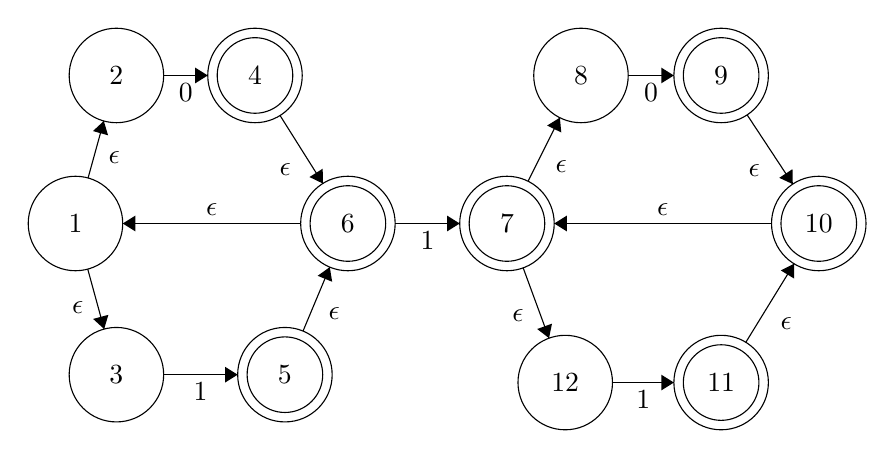
\begin{tikzpicture}[scale=0.2]
\tikzstyle{every node}+=[inner sep=0pt]
\draw [black] (12.5,-16.2) circle (3);
\draw (12.5,-16.2) node {$1$};
\draw [black] (15.1,-6.8) circle (3);
\draw (15.1,-6.8) node {$2$};
\draw [black] (15.1,-25.8) circle (3);
\draw (15.1,-25.8) node {$3$};
\draw [black] (25.8,-25.8) circle (3);
\draw (25.8,-25.8) node {$5$};
\draw [black] (25.8,-25.8) circle (2.4);
\draw [black] (29.8,-16.2) circle (3);
\draw (29.8,-16.2) node {$6$};
\draw [black] (29.8,-16.2) circle (2.4);
\draw [black] (23.9,-6.8) circle (3);
\draw (23.9,-6.8) node {$4$};
\draw [black] (23.9,-6.8) circle (2.4);
\draw [black] (39.9,-16.2) circle (3);
\draw (39.9,-16.2) node {$7$};
\draw [black] (39.9,-16.2) circle (2.4);
\draw [black] (44.6,-6.8) circle (3);
\draw (44.6,-6.8) node {$8$};
\draw [black] (43.6,-26.3) circle (3);
\draw (43.6,-26.3) node {$12$};
\draw [black] (53.5,-6.8) circle (3);
\draw (53.5,-6.8) node {$9$};
\draw [black] (53.5,-6.8) circle (2.4);
\draw [black] (53.5,-26.3) circle (3);
\draw (53.5,-26.3) node {$11$};
\draw [black] (53.5,-26.3) circle (2.4);
\draw [black] (59.7,-16.2) circle (3);
\draw (59.7,-16.2) node {$10$};
\draw [black] (59.7,-16.2) circle (2.4);
\draw [black] (26.8,-16.2) -- (15.5,-16.2);
\fill [black] (15.5,-16.2) -- (16.3,-16.7) -- (16.3,-15.7);
\draw (21.15,-15.7) node [above] {$\epsilon$};
\draw [black] (13.3,-13.31) -- (14.3,-9.69);
\fill [black] (14.3,-9.69) -- (13.61,-10.33) -- (14.57,-10.6);
\draw (14.57,-12.04) node [right] {$\epsilon$};
\draw [black] (13.28,-19.1) -- (14.32,-22.9);
\fill [black] (14.32,-22.9) -- (14.59,-22) -- (13.62,-22.26);
\draw (13.03,-21.52) node [left] {$\epsilon$};
\draw [black] (18.1,-6.8) -- (20.9,-6.8);
\fill [black] (20.9,-6.8) -- (20.1,-6.3) -- (20.1,-7.3);
\draw (19.5,-7.3) node [below] {$0$};
\draw [black] (18.1,-25.8) -- (22.8,-25.8);
\fill [black] (22.8,-25.8) -- (22,-25.3) -- (22,-26.3);
\draw (20.45,-26.3) node [below] {$1$};
\draw [black] (26.95,-23.03) -- (28.65,-18.97);
\fill [black] (28.65,-18.97) -- (27.88,-19.52) -- (28.8,-19.9);
\draw (28.54,-21.93) node [right] {$\epsilon$};
\draw [black] (25.49,-9.34) -- (28.21,-13.66);
\fill [black] (28.21,-13.66) -- (28.2,-12.72) -- (27.36,-13.25);
\draw (26.22,-12.8) node [left] {$\epsilon$};
\draw [black] (32.8,-16.2) -- (36.9,-16.2);
\fill [black] (36.9,-16.2) -- (36.1,-15.7) -- (36.1,-16.7);
\draw (34.85,-16.7) node [below] {$1$};
\draw [black] (41.24,-13.52) -- (43.26,-9.48);
\fill [black] (43.26,-9.48) -- (42.45,-9.98) -- (43.35,-10.42);
\draw (42.95,-12.61) node [right] {$\epsilon$};
\draw [black] (40.93,-19.02) -- (42.57,-23.48);
\fill [black] (42.57,-23.48) -- (42.76,-22.56) -- (41.82,-22.9);
\draw (40.99,-22.05) node [left] {$\epsilon$};
\draw [black] (47.6,-6.8) -- (50.5,-6.8);
\fill [black] (50.5,-6.8) -- (49.7,-6.3) -- (49.7,-7.3);
\draw (49.05,-7.3) node [below] {$0$};
\draw [black] (46.6,-26.3) -- (50.5,-26.3);
\fill [black] (50.5,-26.3) -- (49.7,-25.8) -- (49.7,-26.8);
\draw (48.55,-26.8) node [below] {$1$};
\draw [black] (55.15,-9.3) -- (58.05,-13.7);
\fill [black] (58.05,-13.7) -- (58.03,-12.75) -- (57.19,-13.3);
\draw (55.99,-12.83) node [left] {$\epsilon$};
\draw [black] (55.07,-23.74) -- (58.13,-18.76);
\fill [black] (58.13,-18.76) -- (57.29,-19.18) -- (58.14,-19.7);
\draw (57.24,-22.53) node [right] {$\epsilon$};
\draw [black] (56.7,-16.2) -- (42.9,-16.2);
\fill [black] (42.9,-16.2) -- (43.7,-16.7) -- (43.7,-15.7);
\draw (49.8,-15.7) node [above] {$\epsilon$};
\end{tikzpicture}
\end{figure}

\item
Fie expresia regulată: $0*(1|000*)*0*$. Construiţi automatul finit epsilon care acceptă limbajul definit de această expresie regulată.

Se fac automate finite pentru bucati din expresia regulata : 0* , 1 , 000* . In urma operatiilor de concatenare , reuniune intre automatele mentionate anterior se obtine automatul finit epsilon sub forma finala schitat mai jos.\\\\\\

\begin{figure}[H]
\centering
\begin{tikzpicture}[shorten >=0.5pt,node distance=2cm,on grid,auto]
\node[state,initial,accepting] (0)  {0} ;
\node[state](1)[right of=0] {1};
\node[state](2)[above of=1] {2};
\node[state](3)[right of=2] {3};
\node[state](4)[below right of=1] {4};
\node[state](5)[right of=4] {5};
\node[state](6)[right of=5] {6};
\node[state,accepting](7)[above right of=6] {7};
\node[state,accepting] (8)[below of=7]   {8} ;
\path[->]
 (0)edge[loop above] node {0} (0)
 	edge node {$\epsilon$} (1)
 	edge[bend right] node {$\epsilon$} (8)
 (1)edge node {$\epsilon$} (2)
 	edge node {$\epsilon$} (4)
 (2)edge node {1} (3)
 (3)edge[bend right] node {$\epsilon$} (1)
 	edge node {$\epsilon$} (7)
 (4)edge node {0} (5)
 (5)edge node {0} (6)
 (6)edge[bend right] node {$\epsilon$} (1)
 	edge node {$\epsilon$} (7)
 (7)edge node {$\epsilon$} (8)
 (8)edge[loop right] node {0} (8)
  ;
\end{tikzpicture}
\caption{Automat finit epsilon ex.6}
\end{figure}

\item
Fie expresia regulată: $[a-c^{\wedge}]+\;|\;(abc)? \;|\; \epsilon$. Construiţi automatul finit epsilon care acceptă limbajul definit de această expresie regulată.

\begin{itemize}
\item $[a-c^{\wedge}]+ \equiv (a\;|\;b\;|\;c\;|\;^{\wedge}) +$

Automat care accepta $[a-c^{\wedge}] +$:  

\begin{figure}[H]
\centering
\begin{tikzpicture}[shorten >=1pt,node distance=3cm,on grid,auto]

  \node[state,initial]	(0)		   		{$q_0$};
  \node[state, accepting]   (1)  	[right of=0] 	{$q_1$};  
  
 \path[->]
     (0)	edge 			node	{a,b,c,$^{\wedge}$} (1)
     (1)	edge	[bend left]	node	{$\epsilon$} (0)    
  ;
\end{tikzpicture}
\end{figure}

\item $(abc)? \equiv abc \; | \; \epsilon$\\

Automat care accepta $abc$:  

\begin{figure}[H]
\centering
\begin{tikzpicture}[shorten >=1pt,node distance=3cm,on grid,auto]

  \node[state,initial]	(0)		   		{$q_0$};
  \node[state]    			(1)  	[right of=0] 	{$q_1$};  
  \node[state]    			(2)  	[right of=1] 	{$q_2$};  
  \node[state,accepting]  	(3)  	[right of=2] 	{$q_3$};  

 \path[->]
     (0)	edge 			node	{a} (1)
     (1)	edge			node	{b} (2)
     (2)	edge			node	{c} (3)    
  ;
\end{tikzpicture}
\end{figure}

Automat care accepta $\epsilon$:

\begin{figure}[H]
\centering
\begin{tikzpicture}[shorten >=1pt,node distance=3cm,on grid,auto]

  \node[state,initial,accepting]	(0)		   		{$q_0$};  

 \path[->]

  ;
\end{tikzpicture}
\end{figure}

Automat care accepta $abc \;| \; \epsilon$

\begin{figure}[H]
\centering
\begin{tikzpicture}[shorten >=1pt,node distance=2cm,on grid,auto]

  \node[state,initial]		(0)		   				{$q_0$};
  \node[state]    			(1)  	[right of=0] 	{$q_1$};  
  \node[state]    			(2)  	[right of=1] 	{$q_2$};  
  \node[state]  			(3)  	[right of=2] 	{$q_3$};
  \node[state]  	(4)  	[right of=3] 	{$q_4$};
  \node[state,accepting]  			(5)  	[below right of=4] 	{$q_5$};
  \node[state]  			(6)  	[below right of=0] 	{$q_6$};

 \path[->]
     (0)	edge 			node	{$\epsilon$}	(1)
     		edge	[bend right]	node	{$\epsilon$}	(6)

     (1)	edge			node	{a} (2)
     (2)	edge			node	{b} (3)
     (3)	edge 			node	{c}	(4)   
     (4)	edge			node	{$\epsilon$} (5)
     (6)	edge			node	{$\epsilon$} (5)   
  ;
\end{tikzpicture}
\end{figure}

\item Concatenarea $[a-c^{\wedge}]+ \;|\; (abc)?$

\begin{figure}[H]
\begin{tikzpicture}[shorten >=1pt,node distance=2cm,on grid,auto]

  \node[state,initial]    	(7)  				 	{$q_7$};     
  \node[state]  	(8) 	[above right of=7]	{$q_8$};  	
  \node[state]		(0)			[above right of=8]  {$q_0$};
  \node[state]    			(1)  	[right of=0] 	{$q_1$};  
  \node[state]    			(2)  	[right of=1] 	{$q_2$};  
  \node[state]  			(3)  	[right of=2] 	{$q_3$};
  \node[state] 		 	(4)	 	[below of=3] 	{$q_4$};
  \node[state]  	(5) 		[below right of=7]	{$q_5$};
  \node[state]  	(6) 	[right of=5]	{$q_6$};
  \node[state,accepting]  	(9) 	[below of=4]	{$q_9$};

 \path[->]
     (0)	edge 			node	{a} (1)
     		edge	[bend right]	node	{$\epsilon$}	(4)
     (1)	edge			node	{b} (2)
     (2)	edge			node	{c} (3)    
     (3)	edge			node	{$\epsilon$} (4)
     (4)	edge			node	{$\epsilon$} (9)
     (5)	edge 			node	{a,b,c,$^{\wedge}$} (6)
     (6)	edge	[bend left]		node	{$\epsilon$} (5)
   			edge	[bend right]	node	{$\epsilon$} (9) 
     (7)	edge			node	{$\epsilon$} (8)  
     		edge			node	{$\epsilon$} (5)
	 (8)	edge			node	{$\epsilon$} (0)       		  
  ;
\end{tikzpicture}
\end{figure}

\item Concatenarea $[a-c^{\wedge}]+ \;|\; (abc)? \;|\; \epsilon$

\begin{figure}[H]
\begin{tikzpicture}[shorten >=1pt,node distance=2cm,on grid,auto]

  \node[state,initial]    	(7)  				 	{$q_7$};   
  \node[state]  	(8) 	[above right of=7]	{$q_8$};  		
  \node[state]		(0)			[above right of=8]  {$q_0$};
  \node[state]    			(1)  	[right of=0] 	{$q_1$};  
  \node[state]    			(2)  	[right of=1] 	{$q_2$};  
  \node[state]  			(3)  	[right of=2] 	{$q_3$};
  \node[state] 		 	(4)	 	[below of=3] 	{$q_4$};
  \node[state]  	(5) 		[below right of=7]	{$q_5$};
  \node[state]  	(6) 	[right of=5]	{$q_6$};
  \node[state,accepting]  	(9) 	[below of=4]	{$q_9$};

 \path[->]
     (0)	edge 			node	{a} (1)
     		edge	[bend right]	node	{$\epsilon$}	(4)
     (1)	edge			node	{b} (2)
     (2)	edge			node	{c} (3)    
     (3)	edge			node	{$\epsilon$} (4)
     (4)	edge			node	{$\epsilon$} (9)
     (5)	edge 			node	{a,b,c,$^{\wedge}$} (6)
     (6)	edge	[bend left]		node	{$\epsilon$} (5)
   			edge	[bend right]	node	{$\epsilon$} (9) 
     (7)	edge			node	{$\epsilon$} (8)  
     		edge			node	{$\epsilon$} (5) 
     		edge	[bend right=70]	node	{$\epsilon$} (9)
     (8)	edge			node	{$\epsilon$} (0)		      		 
  ;
\end{tikzpicture}
\end{figure}

Eliminand tranzitiile $\epsilon$ vom obtine automatul determinist cautat.

\begin{figure}[H]
\begin{tikzpicture}[shorten >=1pt,node distance=2cm,on grid,auto]

  \node[state,initial,accepting]	(0)		   		{$q_0$};  
  \node[state]    			(1)  	[above right of=0] 	{$q_1$};  
  \node[state]    			(2)  	[below right of=0] 	{$q_2$};  
  \node[state]  			(3)  	[right of=2] 	{$q_3$};
  \node[state, accepting] 		 	(4)	 	[right of=3] 	{$q_4$};

 \path[->]
	(0)	edge			node	{a,c,b,$^{\wedge}$} (1)
		edge			node	{a}	(2)
     (1)	edge	[loop above]		node	{a,c,b,$^{\wedge}$} (2)   
     (2)	edge			node	{b} (3)
     (3)	edge			node	{c} (4)   
  ;
\end{tikzpicture}
\end{figure}
\end{itemize}

\item
Fie expresia regulată: $(10|[0-2]*|(01)?)+$. Construiţi automatul finit epsilon care acceptă limbajul definit de această expresie regulată.

\begin{figure}[H]
\centering
\begin{tikzpicture}[->,>=stealth',shorten >=1pt,auto,node distance=2.5cm,
                    semithick]
 \node[initial,state]         (0)            {$q13$};
  \node[state]         (4) [ above of=0] {$q4$};
\node[state]         (3) [ above of=4] {$q3$};
 \node[state]         (5) [ right of=4] {$q5$};
 \node[state]         (6) [ right of=5] {$q6$};
 \node[state]         (7) [ right of=6] {$q7$};
 \node[state]         (8) [ below right of=5] {$q8$};
 \node[state,accepting]         (9) [ below of=0] {$q9$};
 \node[state]         (10) [ right of=9] {$q10$};
 \node[state]         (11) [ below right of=10] {$q11$};
 \node[state]         (12) [ below of=9] {$q12$};
 \node[state] 	(13)   [right of=3] {$q0$};
  \node[state]         (1) [ right of=13] {$q1$};
\node[state]         (2) [ right of=1] {$q2$};
 \node[state,accepting]         (14) [ below right of=7] {$q14$};
 \path (0) edge              node {$\epsilon$} (4)
	(0) edge             node {$\epsilon$} (9)
           (4) edge                  node {$\epsilon$} (3)
	(4) edge               node {$\epsilon$} (5)
  	(4) edge     [bend right]             node {$\epsilon$} (8)
 	 (9) edge                  node {0} (10)
  	(9) edge                  node {$\epsilon$} (12)
 	 (10) edge                  node {1} (11) 
 	(11) edge                  node {$\epsilon$} (9)
 	 (3) edge                  node {$\epsilon$} (13)
 	(13) edge                  node {1} (1)
  	(1) edge                  node {0} (2)
 	 (5) edge                  node {0,1,2} (6)
 	 (6) edge                  node {$\epsilon$} (7)
 	 (6) edge    [bend left]              node {$\epsilon$} (5)
 	 (8) edge     [bend right]             node {$\epsilon$} (7)
 	 (7) edge                  node {$\epsilon$} (14)
 	 (2) edge                  node {$\epsilon$} (14)
	(12) edge   [bend right]           node {$\epsilon$} (14);
 \end{tikzpicture}
\end{figure}

\item
Să se demonstreze folosind teorema pompării că limbajul 

L = \{ $a^{i}$ $b^{j}$ $c^{k}$ , i+j=k \}

nu este un limbaj regulat.

w=$a^{N}$ $b^{N}$ $c^{2N}$

 1 $\leq$ |y| $\leq$ N, y $\neq$ $\epsilon$
 
 y = $a^{i}$,  1 $\leq$ y $\leq$ N
 
 |xy| $\leq$ N, x=$a^{j}$
  
i+j $\leq$ N

w=$a^{j}$$a^{i}$($a^{N-(i+j)}$$b^{N}$$c^{2N}$)

pentru q=2 $\Rightarrow$  $w^{`}$=$a^{(N+i)}$$b^{N}$$c^{2N}$, $\forall$ i,  $w^{`}$ $\notin$ L.

$\forall$ i, N+i+N $\neq$ 2N,  1 $\leq$ i $\leq$ N, $\Rightarrow$ limbajul este regulat.

\item
Să se demonstreze folosind teorema pompării că limbajul 

Fie L=\{ a$b^{n}$ $c^{n}$ \}

nu este un limbaj regulat.

N = a$b^{n-1}$ $c^{N}$

y = a$b^{i}$,  1 $\leq$ i $\leq$ N, 0 $\leq$ j $\leq$ N-1.

\textit{Cazul 1}  

x = $\epsilon$ $\Rightarrow$ y=a$b^{i}$, z = $b^{(N-1-i)}$$c^{(N-1)}$

$w^{`}$ = ${(ab^{i})}^{q}$ (  $b^{(N-1-i)}$$c^{(N-1)}$ )

pentru q=0 : $w_{0}^{`}$=$b^{(N-1-i)}$$c^{(N-1)}$ $\nexists$ L.

\textit{Cazul 2}

x= a$b^{j}$ $\Rightarrow$ y=$b^{k}$, z = $b^{(N-1-j-k)}$$c^{(N-1)}$
 
$w^{`}$ = $ab^{j}$${(b^{k})}^{q}$ $b^{(N-1-j-k)}$$c^{N-1}$
 
pentru q=0 : $w_{0}^{`}$= a$b^{i}$$b^{(N-1-j-k)}$$c^{(N-1)}$ $\nexists$ L.



\end{enumerate}

\subsection{Exerciţii propuse}

\textbf{Aplicaţie facultativă}
\begin{itemize}
\item
Implementarea într-un limbaj de programare oarecare a unei aplicaţii care să construiască AFD care acceptă acelaşi limbaj ca şi o expresie regulată dată.
\item
Intrare: Expresia regulată.
\item
Iesire:
\begin{itemize}
\item
Elementele de definiţie ale AF-$\epsilon$ echivalent: alfabetul, mulţimea stărilor, starea iniţială, mulţimea stărilor finale, graful de tranziţie.
\item
Codul care implementează funcţionarea AFD echivalent pentru AF-$\epsilon$ de mai sus.
\end{itemize}
\end{itemize}